\documentclass[11pt]{article}
\usepackage[style=apa]{biblatex}
\DeclareLanguageMapping{english}{english-apa} % Resolve labelyearlabelmonthlabelday errors.
\AtEveryBibitem{\clearfield{note}} % Clear note fields.
\usepackage{listings}
\usepackage{enumitem}
\usepackage{lipsum}
\usepackage[symbol]{footmisc}
\usepackage{graphicx}
\usepackage[capposition=top]{floatrow}
\usepackage{listings}
\usepackage{hyperref}
\usepackage{bibentry}
\usepackage[letterpaper, left=1in,top=1in,right=1in,bottom=1in]{geometry}
\usepackage{setspace}
\usepackage{epstopdf}
\usepackage{amssymb}
\usepackage{lineno}
\usepackage{wrapfig}
\usepackage{amsmath}
\usepackage{array}
\usepackage{color,soul}
\usepackage{tabularx}
\usepackage{rotating}
\usepackage{lscape}
\usepackage{subcaption}
\usepackage{longtable}
\usepackage{siunitx}
\usepackage{appendix}
\usepackage{pdfpages}
\usepackage{titlesec}
\usepackage{mfirstuc}
\usepackage{multirow}
\usepackage{threeparttable}
\usepackage{color,soul}
\usepackage{todonotes}
\usepackage{mathptmx} % almost times new roman font.
\usepackage{arydshln} % Dashed line.


\renewcommand{\baselinestretch}{1.5}
\renewcommand{\thefootnote}{\arabic{footnote}}
\bibliography{../reference/classification.bib}
% \bibliography{../reference/algorithms/ml_algorithms.bib}
\setcounter{tocdepth}{2}
\onehalfspacing

% 

\title{{\textsc{Classification of nonprofit organizations: A supervised machine-learning approach}}}
\author{%
\textsc{Ji Ma and Isha Kanani} \thanks{J.M.: maji@austin.utexas.edu, LBJ School of Public Affairs and RGK Center for Philanthropy and Community Service; I.K.: ishakanani@utexas.edu, School of Information.} \\[1ex] % Your name \thanks{}
\normalsize University of Texas at Austin \\ % Your institution
% \normalsize {Email: maji@austin.utexas.edu} \\ % Your email address
}


\date{\today} % Leave empty to omit a date \today

%----------------------------------------------------------------------------------------

\begin{document}

\maketitle

\begin{abstract}
\noindent This research note reports the use of supervised machine-learning algorithms in classifying the nonprofit organizations in the United States. Mission statements and project descriptions are collected from the 990 forms as text data, and classifications using National Taxonomy of Exempt Entities are collected from the National Center for Charitable Statistics at the Urban Institute. Three text classification algorithms are experimented: Na\"ive Bayes, Random Forest, and Neural Network. The Neural Network classification achieves the best results with an average accuracy of 9*.9\% (standard deviation **), recall *** (standard deviation **), and precision *** (SD **). An open-source Python package \textit{npocat} is developed and shared using the trained algorithms. Future projects are discussed.

% The National Taxonomy of Exempt Entities (NTEE) has been used for classifying the nonprofit organizations in the United States for several decades. However, major countries in the world do not have a classification system for the nonprofit sector. This paper achieves three major goals: 1) devising a machine learning model which can classify the nonprofits using mission statements, 2) inventing a functional classification system which can be applied to different countries, 3) test the accuracy of the model and classification system. We first created a classification system cross different countries by matching existing standards, then compiled the training and testing datasets for China (data from China Foundation Center and Research Infrastructure of Chinese Foundations), United Kingdom (data from ****), and United States (data from National Center for Charitable Statistics and Internal Revenue Service). We finally test the accuracy of major text classification algorithms using country-specific training datasets and a pooled dataset. Implications and limitations are discussed.
\end{abstract}
\clearpage

% \listoftodos
\tableofcontents
\listoftables
\listoffigures
\clearpage

\section{Introduction}

Although the voluntary and philanthropic organizations have long been existent for numerous centuries, the so-called ``nonprofit sector'' was only coined in the 1970s by scholars, policy makers, and nonprofit practitioners. A major reason for assembling the diverse organizations as a conceptual whole is to legitimize the existence of these organizations and the benefits these organizations receive \parencites[54-55]{HallHistoricalOverviewPhilanthropy2006}{BarmanClassificatoryStrugglesNonprofit2013}. From Durkheim's \citeyear{DurkheimElementaryFormsReligious2012} perspective, the order and structure of a society can be reflected by a classification system. The National Taxonomy of Exempt Entities (NTEE) developed by the National Center for Charitable Statistics (NCCS), the most widely used classification system, is one of the efforts legitimizing the existence of nonprofit sector \parencite{Hodgkinsonnewresearchplanning1991,HodgkinsonMappingnonprofitsector1990}. As \textcite[105]{BarmanClassificatoryStrugglesNonprofit2013} cite \textcite[601]{ClarkeSimpleTechnologyComplex1996}: ``The ways in which different entities (people, animals, plants, diseases, etc.) are organized into classificatory groups reveal something of the social, cultural, symbolic, and political contexts within which classifications occur.''

The development of NTEE classifications can date back to the 1980s \parencite[8-9, 11]{HodgkinsonMappingnonprofitsector1990}. In 1982, NCCS assembled a team of experts working on creating a taxonomy for nonprofit organizations. The first draft of the taxonomy, entitled ``National Taxonomy of Exempt Entities'' (NTEE), came out in 1986 and published in 1987. In the early 1990s, NCCS had classified nearly one million nonprofits using NTEE. In 1995, the Internal Revenue Service (IRS) adopted the NTEE coding system, took over the tasks of assigning and maintaining the classifications, and started to release the Business Master File with NTEE codes \parencite{USInternalRevenueServiceExemptOrganizationsBusiness2014,USInternalRevenueServiceIRSStaticFiles2013}.

Two agencies took the task of assigning NTEE codes: NCCS and IRS. Before 1995, NCCS coded nonprofits according to the program descriptions in Part III and VIII of Form 990, supplemented with information from Form 1023 (``Application for Recognition of Exemption'') and additional research \parencite[16]{NationalCenterforCharitableStatisticsGuideUsingNCCS2006}. After 1995, IRS began to issue ``new exempt organizations an NTEE code as part of the determination process,'' and ``the determination specialist assigns an NTEE code to each organization exempt under I.R.C. \S 501(a) as part of the process of closing a case when the organization is recognized as tax-exempt'' \parencite[1]{USInternalRevenueServiceIRSStaticFiles2013}.

The NTEE classifications has been used for numerous practical and academic purposes. For example, it provides a framework on which the social and economic activities of nonprofits can be mapped and compared with other types of organizations in a society \parencite[e.g.,][]{RoegerNonprofitSectorIts2015}. It can also serve as an analytical tool for measuring the organizational capacity in different service domains and inform the practitioners and policymakers in decision-making \parencite{Hodgkinsonnewresearchplanning1991}. Scholars also use NTEE codes for sampling purposes \parencite[e.g.,][]{OktenDeterminantsdonationsprivate2000,CarmanEvaluationCapacityNonprofit2010} or as independent variables \parencite{SloanEffectsNonprofitAccountability2009}. The invention of NTEE also provides a fundamental necessity for comparative international research, facilitating the study of ``global civil society'' \parencite{VakilConfrontingclassificationproblem1997,Salamonsearchnonprofitsector1992,Salamoninternationalclassificationnonprofit1996,HodgkinsonMappingnonprofitsector1990}.

The NTEE classification system, although one of the best we have, still has several drawbacks. First, because it only assign one major category code to an organization, it cannot accurately describe a nonprofit's programs which are usually diverse and across several service domains \parencite[303]{GronbjergUsingNTEEclassify1994}. Although a program classification system was developed later \parencite{LampkinIntroducingNonprofitProgram2001}, it is not widely used probably because it is impractical to assign codes to massive amount of programs. Second, the assignment of NTEE codes is not complete because it is ``based on an assessment of program descriptions contained in Parts 3 and 8 of the Form 990'' and ``program descriptions were only available for some organizations'' \parencite[16]{NationalCenterforCharitableStatisticsGuideUsingNCCS2006}. A recent study found the number of organizations in Washington State with a specific NTEE code could be significantly increased if the mission statements were used for coding \parencite{FyallNTEECodesOpportunities2018}. Third, NTEE codes are static but nonprofit organizations' activities may change over time. Recoding existent NTEE assignments is extremely onerous, and this may be one of the reason that IRS does not have a procedure by which the nonprofits can request the change of their NTEE codes \parencite{USInternalRevenueServiceIRSStaticFiles2013}. In general, the tremendous human labor needed for classification is a prominent challenge, and such challenge is also an evident barrier for improving any classification system.

This research note responds to this challenge by applying supervised machine-learning techniques to nonprofit classification. It made the following contributions: 1) we established a standardized workflow and benchmarks which future studies and industrial applications can build on and compare to; 2) we achieved 77\% average accuracy for classifying the nonprofits into 10 broad categories, and 72\% for the classification of 25 major groups; 3) we made a Python package for classifying nonprofits which can be used by academia for free; 4) we released all source codes and data for replication purposes and future study, this is particularly important since there are many caveats in tuning algorithms.\footnote{Will do this after blind peer-review.} 


% By using supervised machine-learning techniques, this study advanced the NTEE classification system from the following perspective: 1) A series of datasets for training models was developed, 2) the accuracy and efficiency of popular text-classification algorithms were compared, 3) existent empirical studies were replicated to test the validity of our machine-learning approach. According to the results of experimentation, validation, and replication, the combination of \hl{\textit{ABC} algorithm} and trained datasets produced the best results.

\section{Method}

\subsection{Working with Texts and Research Workflow}

Classifying texts is a typical task of automatic content analysis and usually employs three types of methods: dictionary, supervised, and unsupervised methods \parencite[268-269]{GrimmerTextDataPromise2013}. The dictionary methods use a predefined dictionary of words to classifying the texts. Although accurate, this approach is not capable to deal with the variations and contexts of language. The supervised method is an improved solution which uses computer algorithms to ``learn'' the linguistic patters in a dataset classified by human coders. Unlike the dictionary and supervised methods which require predefined categories of interest, unsupervised methods can discover linguistic patters in texts without inputting any knowledge of classification. However, unsupervised method's validity can be problematic because the returned classifications may not be theoretically meaningful. To take the advantage of existing human-coded NTEE classifications, this study employs a supervised approach as indicated by Figure \ref{fig:workflow}.

\begin{figure}
	\centering
	\caption{\textsc{Research workflow}} \label{fig:workflow}
	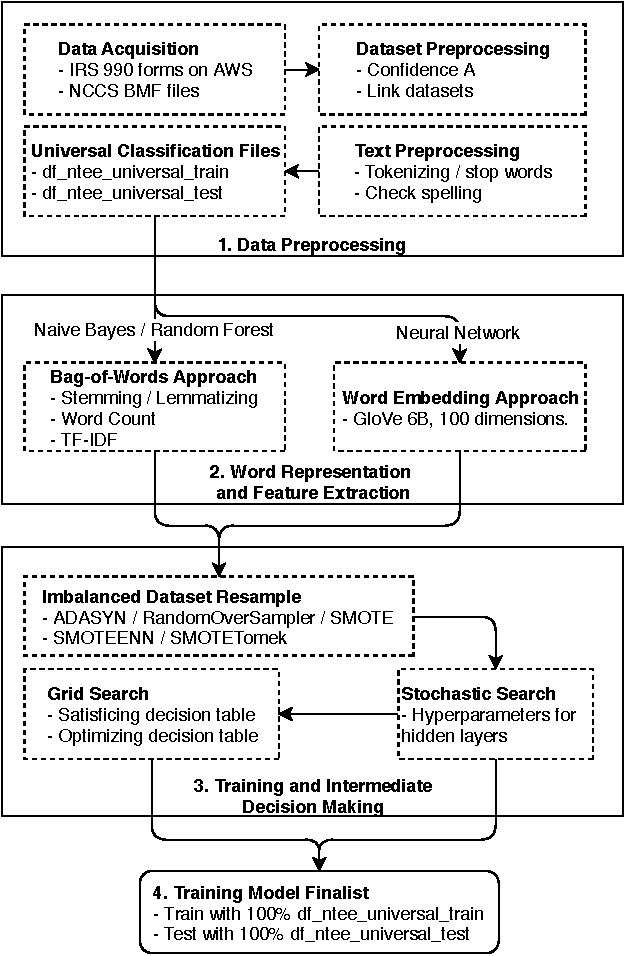
\includegraphics[width=0.7\textwidth]{tbl_fig/ntee_classification.pdf}
\end{figure}

Figure \ref{fig:workflow} shows this paper's complete workflow. We implement four stages of analysis: 1) \textit{preprocessing stage} includes data acquisition and the preprocessing of datasets and texts; 2) \textit{feature extraction} includes bag-of-words (used by Naive Bayes and Random Forest algorithms) and word embedding (used by neural network algorithms); 3) at \textit{training and intermediate decision making} phase, we use stochastic and grid search to train, search, and optimize the machine learning algorithms; 4) we \textit{train the model finalist} with the complete dataset and prepare the trained model for public use. The following part introduces the four phases in detail.

\subsection{Data Preprocessing}

% There are two types of datasets for supervised text classification: training dataset and testing dataset. Both datasets are collections of text records that have been classified by human coders. The machine-learning algorithms can ``learn'' the linguistic patters from the training dataset and then classify the records in testing dataset using the patters learned. The results generated by algorithms can be compared with those coded by human coders, and ultimate goal is to use trained models to replace human. The quality of training dataset is decisive because it must be a representative sample of the whole corpus. The training dataset can be generated by randomly sampling the whole corpus, but a better strategy is proportional sampling according to the distribution of classification scheme \parencite[278]{GrimmerTextDataPromise2013}.

% \subsubsection{Text Data}

\begin{table}[]
    \centering
    \begin{tabularx}{\textwidth}{r|X|X}
    	 \hline
         & Mission Statement & Program Description \\
         \hline
         990 & Part I, Line 1; Part III, Line 1 & Part III, Line 4; Part VIII, Line 2a-e, Line 11a-c; Schedule O \\
         \hdashline
         990-EZ & Part III & Part III, Line 28-30; Schedule O \\
         \hdashline
         990-PF & -- & Part IX-A; Part XVI-B \\
         \hline
    \end{tabularx}
    \caption{\textsc{Locations of text fields in different forms}} \label{tab:text_loc}
    \label{tab:my_label}
\end{table}

\textit{Data acquisition and dataset preprocessing.} We collected text records from form 990, 990-EZ, and 990-PF, and supplemented these records with program descriptions from Schedule O. Form 990 (Return of Organization Exempt From Income Tax) is submitted by most of the nonprofit organizations. For smaller organizations with ``gross receipts of less than \$200,000 and total assets of less than \$500,000 at the end of their tax year'' \parencite[1]{USInternalRevenueService2017InstructionsForm2018}, they can file Form 990-EZ (Short Form Return of Organization Exempt From Income Tax), a shorter version of Form 990. Private foundations use Form 990-PF (Return of Private Foundation). The texts describes organizational activities in two forms: overall mission statement and specific program description. Table \ref{tab:text_loc} summarizes these text fields' specific locations in different forms.

Classification records (i.e., NTEE codes) are collected from the 2014-2016 Business Master Files on NCCS website.\footnote{https://nccs-data.urban.org} This study deals with two types of NTEE classifications: 10 broad category and 26 major groups. Table \ref{tab:classification} shows the relationship between broad categories and major groups. A detail list of the 26 major groups can be found in \textcite{USInternalRevenueServiceExemptOrganizationsBusiness2014}. The accuracy of classification is indicated by a letter of A, B, or C: ``A confidence level of A, for example, indicates that there is at least a 90 percent probability that the major group classification is correct'' \parencite[16]{NationalCenterforCharitableStatisticsGuideUsingNCCS2006}. From 2014 to 2016, 56.12\% records are classified at A level, 37.32\% at B level, and 6.56\% at C level. For training purposes, we only use records at confidence level A and drop all X/Z category (i.e., unknown or unclassified). About 1.76\% organizations changed their NTEE codes between 2014 and 2016. We dropped the records of these organizations since these records are less credible.

\begin{table}[]
    \centering
    \begin{tabularx}{\textwidth}{r|X|X}
    	 \hline
         Broad Category Code & Explanation & Major Group Code \\
         \hline
		I & Arts, Culture, and Humanities & A \\
		II & Education & B \\
		III & Environment and Animals & C, D \\
		IV & Health & E, F, G, H \\
		V & Human Services & I, J, K, L, M, N, O, P \\
		VI & International, Foreign Affairs & Q \\
		VII & Public, Societal Benefit & R, S, T, U, V, W \\
		VIII & Religion Related & X \\
		IX & Mutual/Membership Benefit & Y \\
		X & Unknown, Unclassified & Z \\
         \hline
    \end{tabularx}
    \caption{\textsc{NTEE-CC classification system}} \label{tab:classification}
    \label{tab:my_label}
\end{table}


\textit{Text Preprocessing.} Texts in sentences need to be ``tokenized'' into words before analysis, which is called ``tokenization'' in natural language processing. We also removed stop words (e.g., ``the'', ``a'' and punctuation marks) and checked spelling errors using algorithms based on ``minimum edit distance'' (ie., the minimum number of editing operations needed to change one word into another; \textcite[26]{JurafskySpeechLanguageProcessing2017}).

% A major part of the text available for processing is input by humans.  We all have different writing styles. Also, one word is used in many different ways based on the sentence construction, for example, the word ``paint" can be used as paint, paints, painting and painted, which all mean the same. The algorithm will not automatically discern these words to be the same and this, in turn, will increase the complexity of the text. It is important to normalize the text before giving it for training purpose to reduce the complexity. The normalization process is further divided into three parts.

% \subsubsection{Tokenization}

% The method of breaking the text input into smaller parts is called tokenization, and these parts are called tokens \parencites[57]{manning2014stanford}. Usually, in text classification, each word is treated as an individual token. When defined the separator to be a space `` '', the text between two spaces will be treated as one token, thus a word. We can define separator depending on the text. If we want to tokenize sentences, we can provide the separator to be a full-stop ``.''. In this case, the text between two full-stops, a sentence, will be taken as one token. The natural language toolkit is a widely used toolkit for tokenization in Python \parencites{bird2004nltk}.

\subsection{Word representation and feature extraction}

The machine learning algorithms can only work on numeric vectors that are transformed from the tokenized sentences. A variety of transformation methods can ``represent'' words as vectors, and good methods should be able to easy the process of extracting ``features'' from texts. In general, there are two approaches to word representation: bag-of-words and word embedding.

\subsubsection{Bag-of-words approach}

Bag-of-words approach considers words in texts as mutually independent, as a result, disregards the order of words in text. For example, ``we are health service organization'' and ``health organization service are we'' are the same bag-of-words. This approach serves as the basis for developing many simple language models because it can efficiently represent the possibility of word's occurrence in texts \parencite{BengfortAppliedTextAnalysis2018}. We adopt two methods in this study to represent the texts: count vector and Term Frequency-Inverse Document Frequency.

\textit{Count vector} counts the number of occurrences of all the words in a given text. Given a set of statements, the algorithm first builds an index of all unique words from the collection which is called vocabulary index. The algorithm then represent the texts using words' frequencies and vocabulary index. Table \ref{tab:count_vector} presents a simple example of count vectors, in which ``we focus on education'' is represented as vector $[1, 1, 1, 0, 0, 0, 0]$

\begin{table}
\caption{\textsc{Example of Count Vectors}} \label{tab:count_vector}
\begin{tabular}{m{3.9cm}|m{0.9cm}|m{1cm}|m{0.9cm}|m{1.5cm}|m{1cm}|m{1cm}|m{0.8cm}}
    \hline
    statements X vocabulary & we & focus & on & education & health & care & about \\
    \hline
    we focus on education & 1 & 1 & 1 & 0 & 0 & 0 & 0 \\ 
    \hdashline
    health care care  & 0 & 0 & 0 & 0 & 1 & 2 & 0 \\ 
    \hdashline
    we care about & 1 & 0 & 0 & 0 & 0 & 1 & 1 \\ 
    \hline
\end{tabular}
\end{table}

\textit{Term Frequency-Inverse Document Frequency} (TF-IDF) normalizes raw word frequencies using the number of documents in which the word appears. As Eq. \ref{eq:tfidf} presents, $tf_{ij}$ is the frequency of word $i$ in mission statement $j$, weighted by the inverse document frequency (i.e., $idf_i$; Eq. \ref{eq:idf}), where $N^{total}$ is the number of total mission statements and $N^{i}$ is the number of mission statements that word $i$ appears. The underlying assumption of TF-IDF is that the words appear in all statements are not as important as those occur in a limited number of statements \parencite[278]{JurafskySpeechLanguageProcessing2017}.

\begin{equation} \label{eq:tfidf}
 w_{ij} = tf_{ij} \cdot idf_i 
\end{equation}
\begin{equation} \label{eq:idf}
idf_i = log(\frac{N^{total}}{N^{i}})
\end{equation}

We need to ``normalize'' the texts to reduce the vocabulary size before transforming using either count vector or TF-IDF, because the same word can have numerous spelling variations. For example, ``environments,'' ``environmental,'' and ``environment'' represent the same root word (i.e., \textit{stem}) ``environ.'' Otherwise, the ML models will suffer from ``the curse of dimensionality'': as the feature increases, the data becomes more discrete and less informative to decision making \parencite[94]{BellmanAdaptiveControlProcesses2015}. 

The process of finding stems is called ``morphological parsing'' which includes two primary methods: stemming and lemmatizing \parencite[25]{JurafskySpeechLanguageProcessing2017}. Stemming slices longer strings to smaller ones according to a series of predefined rules. For example, ``ational'' is transformed to ``ate'' in all words ending with the former string. Therefore, stemming tend to have errors of both over- and under-parsing. Lemmatizing is a more advanced method which reduces a word to its stem by analyzing its meaning.

\subsubsection{Word embedding approach}

Disregarding the contexts in which the words appear is an evident drawback of bag-of-words approach. The word embedding approach represents words in a multi-dimensional space (i.e., each word has a vector value), in which words that often appear together in texts have closer distance with each other \parencites[][290]{JurafskySpeechLanguageProcessing2017}[][65]{BengfortAppliedTextAnalysis2018}. We can either train our own word vectors which require a large corpus and is time-consuming, or use pre-trained word vectors. We use the 100-dimension word vectors pre-trained from a corpus of 6 billion word tokens \parencite{PenningtonGloveGlobalVectors2014}.


\subsection{Training and intermediate decision making}

\subsubsection{Classifiers for Training}

\textit{Na\"ive Bayes (NB) classifier} is built on Baye\'s theorem. It is one of the simplest classifiers to learn and implement among all machine learning algorithms and built on simple conditional probability principles. The classifier assumes all features extracted from the texts are conditionally independent, which is wrong in most cases. But the classifier is efficient and has proven to be useful for a variety of tasks even on a small dataset \parencites[][76]{JurafskySpeechLanguageProcessing2017}[][277]{GrimmerTextDataPromise2013}. We tested two types of NB classifiers: multinomial and Complement NB classifiers \parencite{RennieTacklingPoorAssumptions2003}.

% Eq. \ref{bayes} calculates the probability that organization $i$ belongs to a $NTEE$ classification (e.g., ``A'', arts, culture, and humanities), given its text collection $TXT$ defined in Table \ref{tab:text_loc} (i.e., mission statement and program descriptions). 

% \begin{equation} \label{bayes}
%  P(NTEE_i \mid TXT_i) = \frac{P(TXT_i \mid NTEE_i) \, P(NTEE_i)}{P(TXT_i)} 
% \end{equation}

% Na\"ive Bayes classifier   \parencites{lewis1998naive}. So the classifier may not perform well on dependent features.

\textit{Random Forest classification} is implemented by developing multiple prediction models. Each model in this algorithm is trained by different data, and then all of these models are asked to predict for the same record. A prediction class that is elected by most of these small algorithms is given as the prediction result by the random forest algorithm. It uses the word ``forest'' because each small algorithm trained is a decision tree \parencites[83]{QuinlanInductiondecisiontrees1986}. A decision tree represents a set of questions that usually have Yes/No answers. The process starts from the top of the tree with one question, and based on the answer, we further run down on either one side of the tree, and answer another question and repeat till we reach the end of the tree. Each decision tree is trained on a different training set \parencites[124]{BreimanBaggingpredictors1996}. 

Take our study for example, if we provide 5,000 statements with their NTEE codes to a random forest with five trees, each tree will randomly select a thousand records to train. Each tree includes new words at different levels of the tree. For example, the tree starts with word ``emergency,'' it will have two branches for ``yes'' or ``no,'' leading to another word and so on, till the bottom of the tree where the NTEE code is. Since each tree is trained on a different set, when a record is given for prediction, each tree predicts the class independent of other tree. In total of five class predictions will be collected in this case, and the class which has the highest occurrence in the prediction results is given as the final predicted class by the random forest algorithm. 

Since each decision tree in a Random Forest classifier is provided with a unique set of records for the training purpose, it strengthens the performance of the overall forest. The classifier however is difficult to visually interpret. It takes a little effort to visualize how decision trees work and understand the algorithm, unlike the Na\"ive Bayes approach.

\textit{Neural Network (NN) classification} is built on the concepts of a neuron structure of the human mind. Each neuron in the network is connected to a few other neurons of the network by a numerical value called ``weight.'' The neurons process records each one in turn, and learn by looking at their classification (i.e., NTEE code in this case) with the known previous NTEE codes of records. With every new record the neurons learn, they update the connection value ``weight'' to update the model \parencites[163]{CollobertUnifiedArchitectureNatural2008}. After the network is done processing each record of the training set, it has final weights for each connection between two neurons. When a testing set is provided, the neurons use the final weights to predict the NTEE code. Depending on the architecture of the neurons, we can design a variety of NNs (e.g., the basic fully connected, Recurrent, and Long Short-Term Memory). We test the Convolutional NN (CNN) in this study \parencite{ZhangSensitivityAnalysisPractitioners2015}.

NN algorithms beat many other machine learning algorithms in most cases. A significant amount of work available compares the performance of different approaches for the same dataset and neural networks algorithm beats many times. However, the model only works well when the data is in a significant amount. Along with the large size of data, this classification method also consumes a high computation power to train the network. One of the biggest disadvantages of Neural Networks is its ``Black Box Nature'' \parencites{BenitezAreartificialneural1997}, which means that it is difficult to interpret the training process of this approach. There is no pre-defined algorithm that would provide the best results for all data format like text, audio, image etc. Also, the model yielding good accuracy for one text dataset might not give satisfactory results for another text dataset. One has to test different configurations to get the model that works best for the target dataset.

\subsubsection{Measuring performance and intermediate decision making}

\textit{Measuring algorithm performance.} The performance of a classification algorithm can be measured by {accuracy}, {precision}, and {recall}. The \textit{accuracy} measures the percentage of correctly classified organizations as showed in Eq. \ref{accuracy}, where $i$ is one of the three classification algorithms (i.e., NB, RF, and NN), $Org^{correct}$ is the number of organizations correctly classified by the algorithm $i$, and $Org^{total}$ is the total organizations to be classified. For example, $Accuracy^{RF}=0.6$ indicates that, when RF classifies an organization, the chance of getting right is 60\%.

\begin{equation} \label{accuracy}
    Accuracy^i=\frac{Org^{correct}}{Org^{total}}
\end{equation}

The \textit{precision} and \textit{recall} measures the performance of a classifier on a specific category. In Eq. \ref{precision}, $k$ is one of the NTEE codes, $Org^{correct}_{k}$ is the number of organizations correctly classified as $k$ by algorithm $i$, and ${Org^{i}_{k}}$ is the number of organizations classified as $k$ by algorithm $i$. $Org^{correct}_{k}$ will always be smaller than or equal to ${Org^{i}_{k}}$ because ML algorithms can hardly predict everything right. For example, $Precision^{NN}_{B}=0.75$ indicates that 75\% of all the organizations classified as ``education'' by the NN algorithm are correct.

\begin{equation} \label{precision}
    Precision^{i}_{k}=\frac{Org^{correct}_{k}}{Org^{i}_{k}}
\end{equation}

Given a human coder labels an organization as category \textit{k}, the \textit{recall} measures the chance the classifier \textit{i} also identifies the organization as \textit{k}. In Eq. \ref{recall}, $Org^{hum}_{k}$ is the number of organizations that has been classified as $k$ by human coders. For example, $Recall^{NN}_{B}=0.80$ denotes that 80\% of the organizations classified as ``education'' by human coders are correctly identified by the NN algorithm.

\begin{equation} \label{recall}
    Recall^{i}_{k}=\frac{Org^{correct}_{k}}{Org^{hum}_{k}}
\end{equation}

\textit{Intermediate decision making.} Finding the best ML algorithm with appropriate parameters is the goal of this study. We can either try some of the configurations randomly (i.e., \textit{stochastic search}), or iterate all possible configurations (i.e., \textit{grid search}). For NB and RF algorithms, we used the latter approach. For NN algorithms, we first used stochastic search to narrow down the configurations of hidden layers, and then conducted a grid search for the input and output layers' parameters using CNN. The grid search for all possible parameter configurations (over 2 million combinations) is impossible by even using one of the most advanced super computing clusters in the world.

We conduced two rounds of grid search. The first found is for \textit{satisficing decision making} in which we only considered the configurations that can perform at the top 5 percent. Then we ran the second found grid search for \textit{optimizing decision making} in which we increased the values of some parameters to allow the algorithms to reach their performance ceilings. We then choose the best algorithm and parameters for final training.


\section{Results}

CNN classifier achieves the best overall performances for classifying the 10 broad categories and the 25 major groups: 77\% accuracy (precision, recall, F1). Detail satisficing decision table can be found in source code repository published online (\texttt{/output} folder). The accuracy for each category or group varies as showed in Table. This is table important for researchers who may want to use our model to identify certain types of nonprofits for their own research question. For example, researchers focusing on ``Education'' organizations should feel confident that 83\% organizations that classified as broad category II are correct.

The performance of our CNN classier approximate or even outperform that of human coders.


\sloppy
\printbibliography

\end{document}

%%%%%%%%%%%%%%%%%%%%%%%%%%%%%%%%% DRAFT %%%%%%%%%%%%%%%%%%%%%%%%%%%%%%%%%
% \textit{Checking the Train and Test Distributions}

% How to split the data is one of the important decisions made in earlier stages of the development. One of the factor considered here is maintaining the distribution of the data, which means that the training and testing datasets should represent the similar distribution of different classes as the distribution in raw dataset. We ensure the same by sampling the dataset, which randomly selects the observations from raw datasets and puts it into either train or test dataset. Since no manipulation is implemented, the resulting sets are expected to have the similar distribution as the raw dataset. 

% Since our dataset consists of 25 classes and few of these classes also have much smaller number of observation in comparison to other classes, the model can generate bias during the training phase if enough observations are not provided for the smaller classes. To ensure this, a satisficing condition\parencite{charnes1963deterministic} is fixed while sampling the raw data. When a training set is generated, it is made sure that the dataset consists of atleast 250 observations of each class, thus ensuring that the smallest class would also have enough number of training observations. If the condition is not satisifed, the training and testing sample is discarded and the sampling process is implemented again, until the satisficing creteria is matched.

% \textit{Train, Validation, and Test data}
% In order to train the model, and then test the accuracy of it using test data, the data is split into training, valiation, and testing datasets. The data here is split into 70/30 initial ratio, indicating that 70 percent of the data being used for model training and 30 percent data to be used for verifying the results provided by the model.

% For the purpose of grid search, we take random 150000 observations from our dataset as a starting point. We divide this sample into 70 and 30 percent keeping in check with the distribution. 80 percent observations from the 70 percent are fed to the model as training data, and the remaining 20 percent of the same 70 percent is used for the validation purpose for the models. When the model gives it's final statistics, we verify validation accuracy of the model using the 30 percent data that we kept apart initially.

% For the purpose of next round of model development, we take our whole dataset. 80 percent of the whole dataset is used as training data for the model, again checking with the distribution consistency. The remaining 20 percent is also fed to the model, for validation purposes.

% grid search: Conv1D(num_filters, kernel_size, activation=conv_act)
% output dense layer activation: out_act
% num_filters: 32, 64, 128
% kernel_size: 3, 5, 7
% conv_act & out_act: 'sigmoid', 'softplus', 'tanh', 'softmax'

%results[(results['val_acc']>0.7) & (results['acc']>0.75)]
% output: conv_act: softplus, out_act: softplus, sigmoid, softmax
% conv_num_filters: 64, 128
% kernel_size: 3

% For the Neural Network Convolutional algorithm, a grid search is first implemented. This grid search puts different values to the parameters of Conv1D layer of keras and the output activation function of the Dense layer. Each model is trained for 50 epochs. In total of 7200 results are obtained by evaluating the model at each epoch. Performance measures recorded include accuracy, validation accuracy, loss, and validation loss. 

%results.sort_values('val_acc', ascending=False).drop_duplicates(["conv_act","out_act", "conv_num_filters", "conv_kernel_size"])
%144 results
% head_count = int(len(final_matrix)*0.05) + 1
%final_matrix = final_matrix.head(head_count)

% The 7200 results are grouped by unique conv act,out act, conv num filters, and conv kernel size, and from 50 epoches for each, the one with the highest validation accuracy is selected. This results into total of 144 results. The validation accuracy is set here to be the satisficing metric and top 5 percent of the records with highest validation accuracy are selected. The process ends up into 8 results of different combinations.

% \begin{figure}
% 	\centering
% 	\caption{\textsc{Decision Making}} \label{fig:decisionmaking}
% 	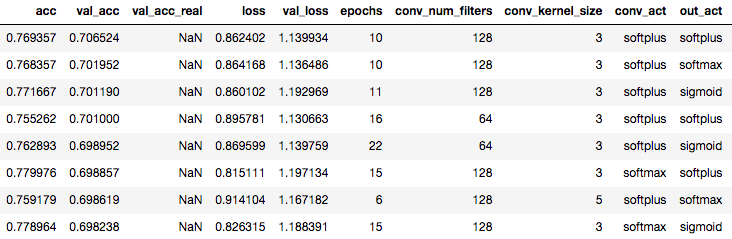
\includegraphics[width=1\textwidth]{tbl_fig/decision_making.png}
% \end{figure}

% The results give convolutional number of filters to be 128 in 6 out of 8 cases, and kernel size of 3 for 7 out of 8 results. The combinatons of convolutional activation and output dense activation include softplus and softplus, softplus and softmax, softplus and sigmoid, softmax and softplus, and softmaz and sigmoid.



% In the context of text classification: Na\"ive Bayes classifier needs a set of features as input, hence we need to provide our text in the form of a set that consists of words from the text. This representation is called bag-of-words \parencites{Jurafsky:2009:SLP:1214993}, which consists of all important words from the text, and the number of times each word occurs in the text. 



% In the training data set, each ``text'' is converted to a bag-of-words where the mission statement is converted into the set of words and given as an input. Along with the input, the output class ``label'' is also provided for the training purpose. The classifier links each input set with its corresponding output class and trains itself. For testing purpose, the classifier is given a bag-of-words as input and asked to predict the class with the highest probability for the given set of words.







% Algorithms perform different mathematical functions on the given input data. These functions need numbers to work on them. Usually, these numbers are given in a table format called a vector. The algorithms perform mathematical functions like multiplication on given vectors for the training purpose. The data we have here is not originally in numerical format, and hence our text cannot be given in the string format to the algorithm. We need to convert our texts into a table format that represents numerical data. This process is called vectorization. 





% \begin{figure}
% \caption{Draft to be modified}
% \label{classification_algo}
% \centering
% 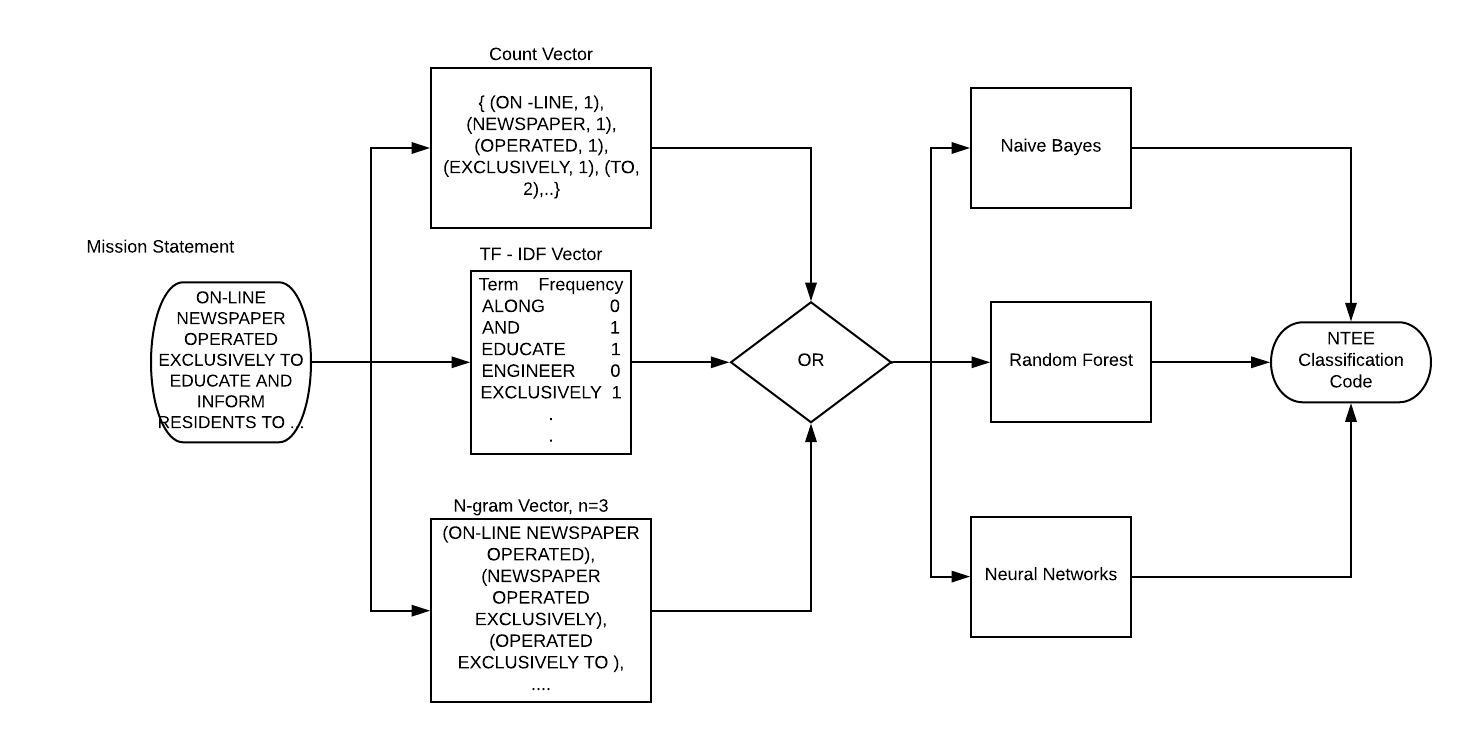
\includegraphics[width=\textwidth]{reference/algorithms/classification_algo.jpeg}
% \end{figure}